% Foliensatz: "AFu-Kurs nach DJ4UF" von DK0TU, Amateurfunkgruppe der TU Berlin
% Lizenz: CC BY-NC-SA 3.0 de (http://creativecommons.org/licenses/by-nc-sa/3.0/de/)
% Autoren: Martin Deutschmann <martin.deutschmann@campus.tu-berlin.de>
% Korrekturen: Lars Weiler <dc4lw@darc.de>, Sebastian Lange <dl7bst@dk0tu.de>

\documentclass[aspectratio=169]{beamer}

\usepackage[ngerman]{babel} % deutsche Worttrennung etc.
\usepackage[utf8]{inputenc} % UTF8 Text

\usepackage[super, comma, numbers, square, sort]{natbib}

\usepackage{hyperref}       % Hyperref Package für bessere Referenzen (todo)
\hypersetup{
	colorlinks=false,       %   false: boxed links; true: colored links
    %linkcolor=white,       %   color of internal links (change box color with linkbordercolor)
    citecolor=red,          %   color of links to bibliography
    filecolor=white,        %   color of file links
    urlcolor=blue           %   color of external links
}

\usepackage{multirow}
\usepackage{wasysym}  % Math Symbols like \permil
%\usepackage{colortbl}
%\usepackage{subscript}
%\usepackage{caption}
%\usepackage{setspace}
%\usepackage{xcolor}        % benutze CodeListe

% Footnote
%\usepackage{hanging}
%
%\setbeamertemplate{footnote}{%
%  \hangpara{2em}{1}%
%  \makebox[2em][l]{\insertfootnotemark}\footnotesize\insertfootnotetext\par%
%}


%\usepackage{pgf}
%\usepackage{tikz}
%\usetikzlibrary{arrows,automata}
%\usetikzlibrary{positioning}
%
%\tikzset{
%    state/.style={
%           rectangle,
%           rounded corners,
%           draw=black, very thick,
%           minimum height=2em,
%           minimum width=2pt,
%           inner sep=2pt,
%           text centered,
%           },
%}

%\usepackage{listings}
%\lstset{basicstyle=\small, numberstyle=\tiny, extendedchars=true, numbers=left, numbersep=5pt}
%\lstset{showtabs=false, showspaces=false, showstringspaces=false}
%%\lstset{backgroundcolor=\color{white!75!lightgray}, , frame=single}
%%\lstset{backgroundcolor=\color{white}}
%%\lstset{backgroundcolor=none}
%\lstset{keywordstyle=\color{blue!50!gray},  identifierstyle=\color{black}}
%\lstset{commentstyle=\color{green!50!gray}, stringstyle=\color{red!50!gray}}
%\lstset{language=C, fontadjust=true, tabsize=2, breaklines=true}
%\lstset{backgroundcolor=\color{white!75!lightgray}, caption=\lstname, frame=single}
%\lstset{emphstyle=\color{black}\fbox}
%
%% Keine "Listing:"-Caption
%\captionsetup{labelformat=empty,labelsep=none}
%
%% für mathematische Umgebungen
%\usepackage{amsmath,amsfonts,amssymb}
%
%\lstdefinestyle{Bash}{
%language=Bash,
%frame=single,
%rulecolor=\color{black},
%backgroundcolor=\color{gray!50},
%keywordstyle=\color{black},
%identifierstyle=,
%commentstyle=\color{black},
%stringstyle=\color{magenta!65!white},
%showstringspaces=false,
%basicstyle=\footnotesize\ttfamily\color{black},
%numbers=none,
%breaklines=true,
%captionpos=b
%}

%\usepackage{listings}
%
%\lstdefinestyle{basic}{
%    captionpos=t,%
%    basicstyle=\footnotesize\ttfamily,%
%    numberstyle=\tiny,%
%    numbers=left,%
%    stepnumber=1,%
%    frame=single,%
%    showspaces=false,%
%    showstringspaces=false,%
%    showtabs=false,%
%    %
%    keywordstyle=\color{blue},%
%    identifierstyle=,%
%    commentstyle=\color{gray},%
%    stringstyle=\color{magenta}%
%}



% fließende Boxen haben keinen Abstand
%\fboxsep0mm

% inkludiere Creative Commons Helper
%%%%%%%%%%%%%%%%%%%%%%%%%%%%%%%%%%%%%%%%%%%%%%%%%%%%%%%%%%%%%%%%
%% ccBeamer 0.1, 2007-07-02                                   %%
%% Written by Sebastian Pipping <webmaster@hartwork.org>      %%
%% ---------------------------------------------------------- %%
%% Licensed under Creative Commons Attribution-ShareAlike 3.0 %%
%% http://creativecommons.org/licenses/by-sa/3.0/             %%
%%%%%%%%%%%%%%%%%%%%%%%%%%%%%%%%%%%%%%%%%%%%%%%%%%%%%%%%%%%%%%%%


%% Images
\newcommand{\CcImageBy}[1]{%
	
\includegraphics[scale=#1]{texdata/creative_commons/cc_by_30.pdf}%
}
\newcommand{\CcImageCc}[1]{%
	
\includegraphics[scale=#1]{texdata/creative_commons/cc_cc_30.pdf}%
}
\newcommand{\CcImageDevNations}[1]{%
	
\includegraphics[scale=#1]{texdata/creative_commons/cc_dev_nations_30.pdf}%
}
\newcommand{\CcImageNc}[1]{%
	
\includegraphics[scale=#1]{texdata/creative_commons/cc_nc_30.pdf}%
}
\newcommand{\CcImageNd}[1]{%
	
\includegraphics[scale=#1]{texdata/creative_commons/cc_nd_30.pdf}%
}
\newcommand{\CcImagePd}[1]{%
	
\includegraphics[scale=#1]{texdata/creative_commons/cc_pd_30.pdf}%
}
\newcommand{\CcImageSa}[1]{%
	
\includegraphics[scale=#1]{texdata/creative_commons/cc_sa_30.pdf}%
}
\newcommand{\CcImageSampling}[1]{%
	
\includegraphics[scale=#1]{texdata/creative_commons/cc_sampling_30.pdf}%
}
\newcommand{\CcImageSamplingPlus}[1]{%
	
\includegraphics[scale=#1]{texdata/creative_commons/cc_sampling_plus_30.pdf}%
}


%% Groups
\newcommand{\CcGroupBy}[2]{% zoom, gap
	\CcImageCc{#1}\hspace*{#2}\CcImageBy{#1}%
}
\newcommand{\CcGroupByNc}[2]{% zoom, gap
	\CcImageCc{#1}\hspace*{#2}\CcImageBy{#1}\hspace*{#2}\CcImageNc{#1}%
}
\newcommand{\CcGroupByNcNd}[2]{% zoom, gap
	\CcImageCc{#1}\hspace*{#2}\CcImageBy{#1}\hspace*{#2}\CcImageNc{#1}\hspace*{#2}\CcImageNd{#1}%
}
\newcommand{\CcGroupByNcSa}[2]{% zoom, gap
	\CcImageCc{#1}\hspace*{#2}\CcImageBy{#1}\hspace*{#2}\CcImageNc{#1}\hspace*{#2}\CcImageSa{#1}%
}
\newcommand{\CcGroupByNd}[2]{% zoom, gap
	\CcImageCc{#1}\hspace*{#2}\CcImageBy{#1}\hspace*{#2}\CcImageNd{#1}%
}
\newcommand{\CcGroupBySa}[2]{% zoom, gap
	\CcImageCc{#1}\hspace*{#2}\CcImageBy{#1}\hspace*{#2}\CcImageSa{#1}%
}
\newcommand{\CcGroupDevNations}[2]{% zoom, gap
	\CcImageCc{#1}\hspace*{#2}\CcImageDevNations{#1}%
}
\newcommand{\CcGroupNcSampling}[2]{% zoom, gap
	\CcImageCc{#1}\hspace*{#2}\CcImageNc{#1}\hspace*{#2}\CcImageSampling{#1}%
}
\newcommand{\CcGroupPd}[1]{% zoom
	\CcImagePd{#1}%
}
\newcommand{\CcGroupSampling}[1]{% zoom
	\CcImageSampling{#1}%
}
\newcommand{\CcGroupSamplingPlus}[1]{% zoom
	\CcImageSamplingPlus{#1}%
}


%% Text
\newcommand{\CcLongnameBy}{Attribution}
\newcommand{\CcLongnameByNc}{Attribution-NonCommercial}
\newcommand{\CcLongnameByNcNd}{Attribution-NoDerivs}
\newcommand{\CcLongnameByNcSa}{Attribution-NonCommercial-ShareAlike}
\newcommand{\CcLongnameByNd}{Attribution-NoDerivs}
\newcommand{\CcLongnameBySa}{Attribution-ShareAlike}

\newcommand{\CcNote}[1]{% longname
	This work is licensed under the \textit{Creative Commons #1 3.0 License}.%
}


% generelles Thema auswählen
\usetheme{Goettingen} %Berlin spart ohne Sidebar allerdings angenehm Platz
% AnnArbor | Antibes | Bergen | Berkeley | Berlin | Boadilla | boxes | CambridgeUS | Copenhagen | Darmstadt | default | Dresden | Frankfurt | Goettingen | Hannover | Ilmenau | JuanLesPins | Luebeck | Madrid | Malmoe | Marburg | Montpellier | PaloAlto | Pittsburgh | Rochester | Singapore | Szeged | Warsaw

% Farben wählen
\usecolortheme{beetle}
% beaver | beetle | crane | default | dolphin | dove | fly | lily | orchid | rose | seagull | seahorse | sidebartab | structure | whale | wolverine

% Setze alle Farben auf Grau und Weiß
%\definecolor{craneorange}{RGB}{64,64,64}
%\definecolor{craneblue}{RGB}{255,255,255}

% Schriftart wählen
\usefonttheme{default}
% default | professionalfonts | serif | structurebold | structureitalicserif | structuresmallcapsserif

% Innere Themen(Kopf-, Fuß-, Sidebar usw)
%\useinnertheme{default}
\useinnertheme{circles}
% default | inmargin | rectangles | rounded | circles

% Äußere Themen (Anordnung der inneren, grenzen der Folien etc.)
\useoutertheme{infolines}
% default | infolines | miniframes | shadow | sidebar | smoothbars | smoothtree | split | tree

% Deaktiviere Navigations-Symbole ({} -> leer)
\setbeamertemplate{navigation symbols}{}
%\setbeamertemplate{navigation symbols}{\large \ifnum \insertframenumber <10 0\fi\insertframenumber/\inserttotalframenumber\vspace*{0.2ex}}

% Zeige ein Hintergrundbild
\setbeamertemplate{background canvas}{
        \hspace*{-2.0cm}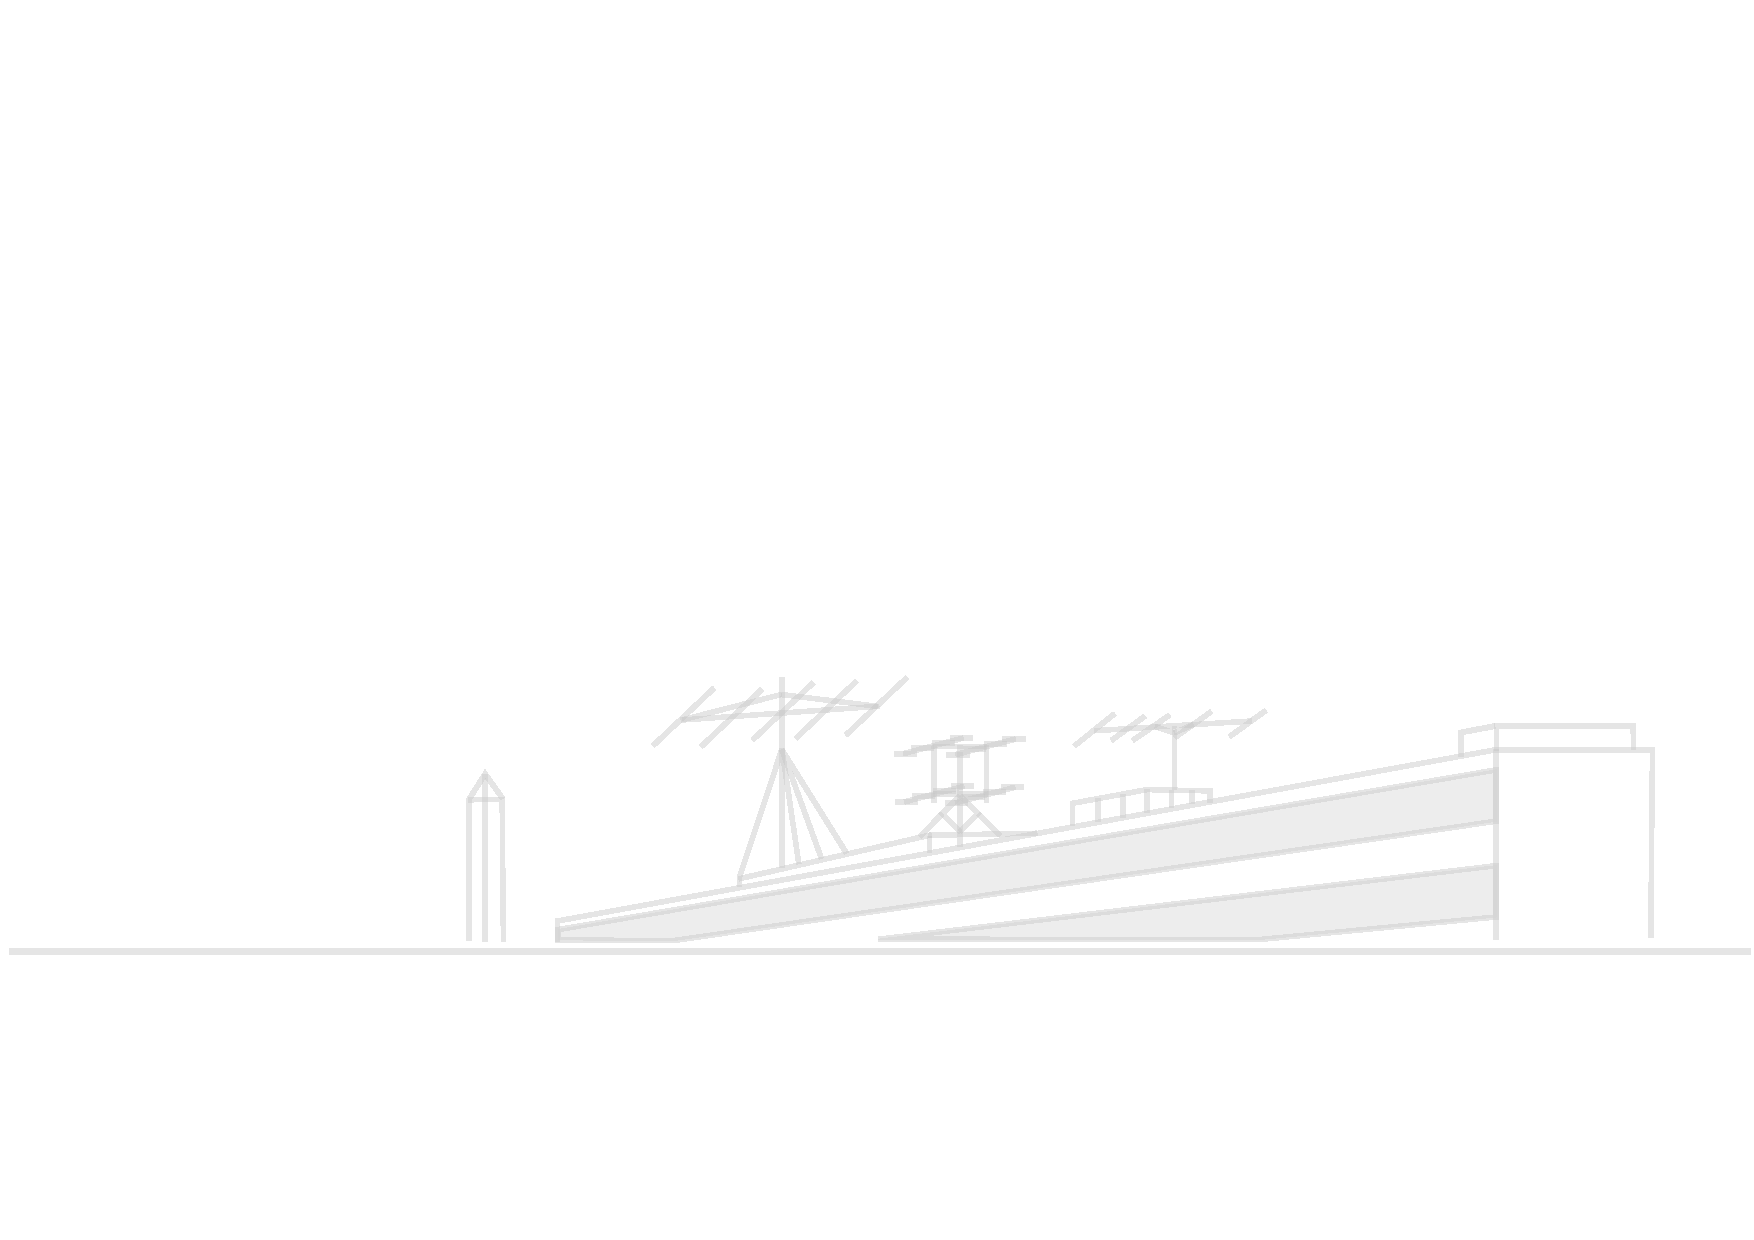
\includegraphics[width=17.8cm]{texdata/dk0tu_rooftop_background.pdf}
}

% Foliennummer einfügen
\setbeamertemplate{footline}[frame number]
%\setbeamertemplate{footline}{}

% Ändere das Zeichen vor jedem item
%\setbeamertemplate{itemize item}{\color{craneorange}$\blacktriangleright$}
%\setbeamertemplate{itemize subitem}{\color{craneorange}$\triangleright$}
%\setbeamertemplate{itemize subsubitem}{\color{craneorange}$\blacktriangleright$}

% Ändert die Blöcke 
\setbeamertemplate{blocks}[rounded][shadow=true]
% default | rounded [shadow=true|false]

%
% Eigene Kommandos
%

% Hack to get natbib and beamer working together. "The beamer user guide suggests
% that only the manual bibliography entry approach is supported"
% on some system it works out of the box, sometimes you need the hack :-(
% so check it --dl7bst
\ifdefined\newblock
    \relax
\else
    \newcommand{\newblock}{}
\fi

% \includedia command to generate png out of a dia file
% NEEDS installed dia and pdflatex option --shell-escape
\newcommand{\includedia}[1]{
    \immediate\write18{/usr/bin/dia #1.dia -e #1_diatmp.png -t png}
}

% RICHIG GROSSER FONT!
\newfont{\bigfont}{cmr10 at 144pt}
\newfont{\smallfont}{cmr10 at 8pt}

% Römische Ziffern
\makeatletter
\newcommand{\rmnum}[1]{\romannumeral #1}
\newcommand{\Rmnum}[1]{\expandafter\@slowromancap\romannumeral #1@}
\makeatother

% Schwarze Überschrift
%\setbeamercolor{frametitle}{fg=black}
%\setbeamercolor{title}{fg=black}

% Item- und Box-Farben
\definecolor{deepBlue}{HTML}{000066}
\setbeamercolor{itemize item}{fg=deepBlue}
\setbeamercolor{itemize subitem}{fg=deepBlue}
\setbeamercolor{description item}{fg=deepBlue}
\setbeamercolor{block title}{fg=deepBlue!100, bg=blue!15}
\setbeamercolor{block body}{fg=black, bg=blue!5}
\setbeamercolor{block title alerted}{fg=deepBlue, bg=red!75}
\setbeamercolor{block body alerted}{fg=black, bg=red!15}
\setbeamercolor*{block title example}{fg=blue!50, bg=blue!10}
\setbeamercolor*{block body example}{fg= blue, bg=blue!5}

%\setbeamercolor{section in head/foot}{parent=palette primary}
%\setbeamercolor{subsection in head/foot}{parent=palette secondary}
%\setbeamercolor{sidebar}{fg=darkblue,bg=yellow!90!orange}
%\setbeamercolor{title in sidebar}{fg=darkblue}
%\setbeamercolor{author in sidebar}{fg=darkblue}
%\setbeamercolor{section in sidebar}{fg=darkblue!10!black}
%\setbeamercolor{subsection in sidebar}{fg=darkblue!50!black}

% Titlepage Infos
\title{AFu-Kurs nach DJ4UF}
\author[DKØTU]{DKØTU\\ \footnotesize{Amateurfunkgruppe der TU Berlin}}
\institute[DKØTU]{\url{http://www.dk0tu.de} }

% PDF-Eigenschaften
\subject{DK0TU-Amateurfunkkurs nach DJ4UF}
\keywords{Amateurfunk Kurs HAM Radio Course CC-BY-NC-SA OpenSource TU Berlin DK0TU}

\subtitle{Technik Klasse A 02: \\
Der Widerstand und seine Schaltungsarten \\[2em]}
\date{Stand 28.04.2016}
 \begin{document}

\begin{frame}
    \titlepage
    \vfill
    \begin{center}
        \ccbyncsaeu\\
        {\tiny This work is licensed under the \em{Creative Commons Attribution-NonCommercial-ShareAlike 3.0 License}.}\\[0.5ex]
         \tiny Amateurfunkgruppe der Technische Universität Berlin (AfuTUB), DKØTU
         %\includegraphics[scale=0.5]{img/DK0TU_Logo.pdf}
    \end{center}
\end{frame}


%fixme Referenzen/Fußnoten-Systematik vereinheitlichen

\section{Einleitung}

\begin{frame}
  \frametitle{Einleitung / Widerstand}
  \begin{center}
    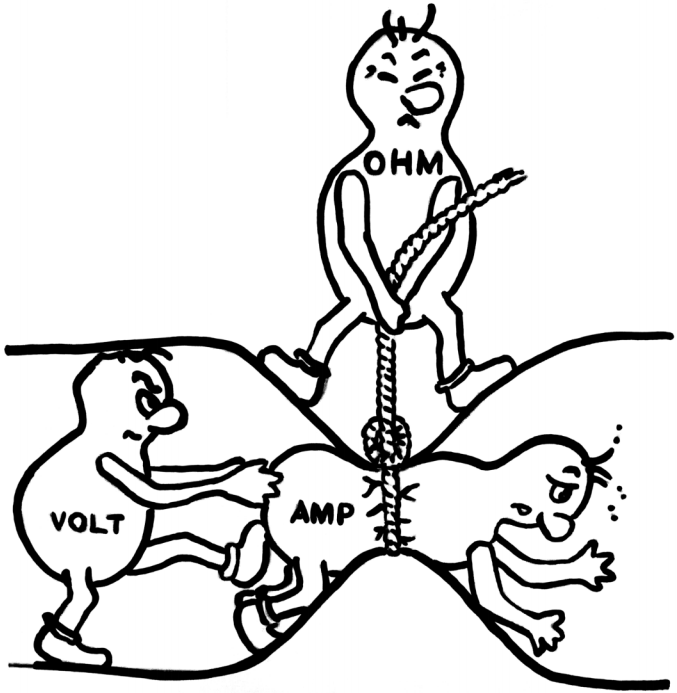
\includegraphics[width=.7\textwidth,height=.8\textheight,keepaspectratio]{e04/URI.png}
    \footnote{\tiny TU Wien \url{http://www.fet.at/twiki/pub/Homepage/OnlineFetzn/fetzn_ausgabe_maerz-2013_online.pdf}}
  \end{center}
\end{frame}


\begin{frame}
  \frametitle{Einleitung / Widerstand}

  \begin{center}
    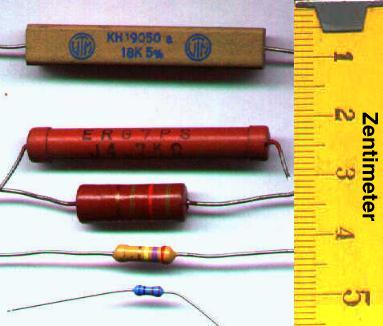
\includegraphics[width=0.8\textwidth,height=.8\textheight,keepaspectratio]{e04/Widerstaende.jpg}
    \footnote{\tiny By Honina at de.wikipedia. Later version(s) were uploaded by Montauk at de.wikipedia.}
  \end{center}

  % TODO SMD-Bauteile ergaenzen

\end{frame}

\begin{frame}
  \frametitle{Einleitung / Widerstand}

  \begin{center}
    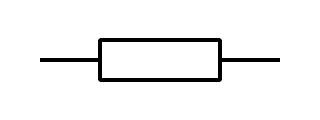
\includegraphics[width=.4\textwidth,height=.2\textheight,keepaspectratio]{e04/Resistor_symbol_IEC.png}
    \footnote{\tiny By Markus Kuhn (Made in Inkscape from scratch) [Public domain], via Wikimedia Commons}
  \end{center}

  \begin{center}
    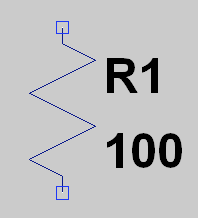
\includegraphics[width=.4\textwidth,height=.5\textheight,keepaspectratio]{e04/R_LTspice.png}
    \footnote{\tiny aus LTspice}
  \end{center}
\end{frame}

\begin{frame}
  \frametitle{Aufbau von Widerständen}
  \textbf{Kohleschichtwiderstände:}
  \pause
  \begin{itemize}
    \item Günstig in der Herstellung
    \item Hohe Toleranzen
  \end{itemize}
  \pause
  \textbf{Metallschichtwiderstände:}
  \pause
  \begin{itemize}
    \item Sehr präzise
  \end{itemize}
  \pause
  \textbf{Metalloxidwiderstände:}
  \pause
  \begin{itemize}
    \item HF tauglich
  \end{itemize}
  \pause
  \textbf{Drahtwiderstände:}
  \pause
  \begin{itemize}
    \item Leistungswiderstände für NF
  \end{itemize}
\end{frame}

\section{Spezifischer Widerstand}

\begin{frame}
  \frametitle{Leitende Materialien}
  \begin{columns}
    \column{.6\textwidth}
    \begin{tabular}{llr}
      Material & \multicolumn{2}{r}{Spezifischer Widerstand $\rho$ in $\frac{\Omega \cdot mm^2}{m}$} \\ \hline
      Silber & & $1,587 \cdot 10^{-2}$ \\
      Kupfer & & $1,721 \cdot 10^{-2}$ \\
      Gold & & $2,214 \cdot 10^{-2}$ \\
      Aluminium & & $2,65 \cdot 10^{-2}$ \\
      Zinn & & $1,15 \cdot 10^{-1}$ \\
      Blei & & $2,08 \cdot 10^{-1}$ \\
      Quecksilber & & $9,412 \cdot 10^{-1}$ \\
      Germanium & \only<2>{$\leftarrow$ \textbf{Halbleiter}} & $4,6 \cdot 10^{5}$\\
      Porzellan & \only<2>{$\leftarrow$ \textbf{Isolator}} & $1 \cdot 10^{18}$ \\
    \end{tabular}

    \column{.35\textwidth}
    \only<3>{
    \begin{block}{Berechnung des Widerstands}
      $$R = \rho \cdot \frac{\ell}{A}$$
    \end{block}
    }
  \end{columns}
\end{frame}

\section{Skin-Effekt}

\begin{frame}
  \frametitle{der Skin-Effekt}
  \begin{itemize}
    \item Tritt bei höherfrequenter Wechselspannung auf
    \item Verdrängt die Elektronen aus dem Leitungsinneren an die Leiteroberfläche
    \item Dadurch steigt der Widerstand im Leiter
  \end{itemize}
\end{frame}

\begin{frame}
  \frametitle{Ursachen des Skin-Effektes}
  \begin{center}
    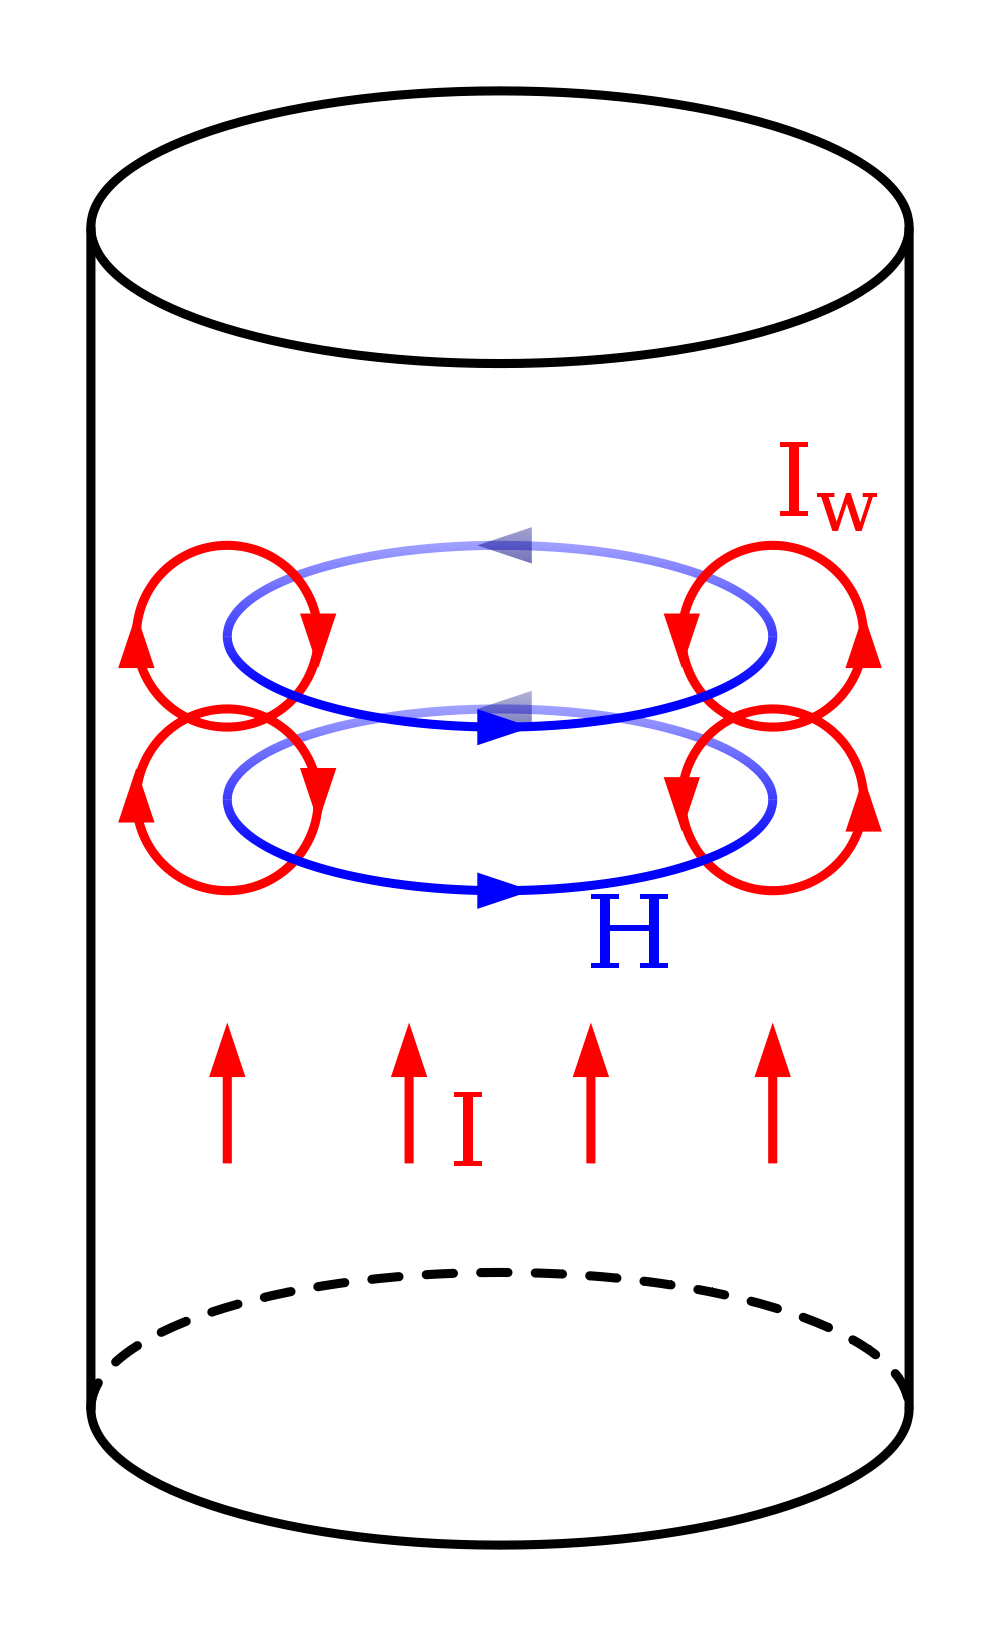
\includegraphics[scale=0.06]{a02/Skineffect.png}\\
    \small{Abb.5: Überlagerung von Wechsel- und Wirbelströmen \cite{wp}}
    \begin{itemize}
      \item Ursache des Skin-Effektes ist das magnetische Feld
      \item Es erzeugt Wirbelströme im Innern des Leiters
      \item Diese sind dem Erzeugerstrom entgegengerichtet
      \item Das wechselnde Magnetfeld erzeugt im Leiter eine höhere Gegenspannung als am Rand
    \end{itemize}
  \end{center}
\end{frame}

\begin{frame}
  \frametitle{Folgen \& Gegenmaßnahmen}
  \textbf{Folgen:}
  \begin{itemize}
    \item Der Leiterquerschnitt sinkt
    \item Die Impedanz steigt
  \end{itemize}
  \textbf{Gegenmaßnahmen}
  \begin{itemize}
    \item Verwendung von Hohlleitern
    \item Mehrere voneinander isolierte Drähte nutzen
    \item Oberfläche versilbern
  \end{itemize}
\end{frame}

\section{Ohmsches Gesetz}

\begin{frame}
  \frametitle{Was ist das ohmsche Gesetz?}
  \begin{itemize}
    \item Das ohmsche Gesetz ist folgendes:
  \end{itemize}
  \begin{center}
    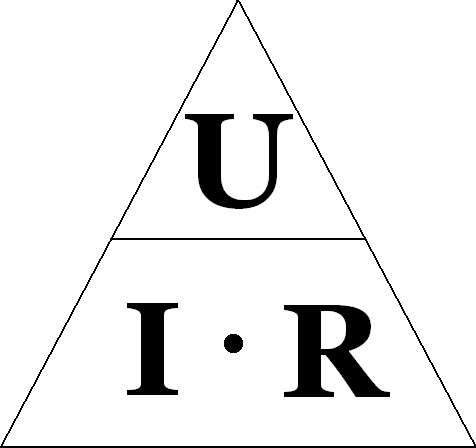
\includegraphics[width=.5\textwidth,height=.6\textheight,keepaspectratio]{e03/Ohm_law_triangle.png}\\
    \small{Abb.6: das ohmsche Dreieck \cite{wmen}}
  \end{center}
  \begin{itemize}
    \item	Aber was sagt uns das nun?
  \end{itemize}
\end{frame}

\begin{frame}
  \frametitle{Das ohmsche Gesetz}
  \begin{itemize}
    \item	Das ohmsche Gesetz gibt uns die Abhängigkeiten zwischen Spannung, Strom \& ohmschen Widerstand an
    \item	Dadurch wissen wir, dass sich zum Beispiel der Strom an einem konstanten Widerstand proportional zur Spannung ändert
  \end{itemize}
\end{frame}

\begin{frame}
  \frametitle{Der Innenwiderstand}
  \begin{itemize}
    \item	Oftmals bemerken wir einen Spannungsabfall zwischen einer Maschine im Leerlauf und der gleichen Maschine bei Belastung
    \item	Dies führen wir auf den Innenwiderstand der Maschine zurück
  \end{itemize}
  \begin{center}
    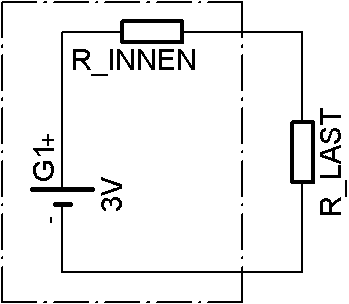
\includegraphics[scale=1.4]{e03/Innenwiderstand.png}\\
    \small{Abb.7: Innenwiderstand einer Batterie}
  \end{center}
\end{frame}

\begin{frame}
  \frametitle{der Innenwiderstand}
  \begin{itemize}
    \item	Um den Innenwiderstand zu ermitteln nutzen wir wieder das ohmsche Gesetz
    \item	Dabei gilt es zu beachten, dass diesmal die Differenzen der Spannungen und des Stromes zwischen dem Leerlauf und dem belasteten Fall verrechnet werden
    \item	Es gilt:
  \end{itemize}
  \begin{block}{Innenwiderstand}
    \begin{center}
      $R_{innen} = \cfrac{\Delta U}{\Delta I}$
    \end{center}
  \end{block}
  \begin{itemize}
    \item	Um den Wert nicht zu sehr zu verfälschen sollten \textbf{Spannungsquellen einen niedrigen} und \textbf{Stromquellen einen hohen Innenwiderstand} besitzen
  \end{itemize}
\end{frame}

% FIXME + Leistungsanpassung, Strom-/Spannungsanpassung Innenwiderzustand zu Lastwiderstand

\section{Rechnen mit Widerständen}

\subsection{Reihenschaltung}
\begin{frame}
  \frametitle{Reihenschaltung}

  \begin{columns}
    \column{.4\textwidth}
    \begin{center}
      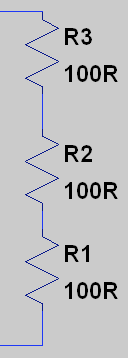
\includegraphics[width=.4\textwidth]{e04/Reihe.png}\footnotemark
    \end{center}
    \pause
    \column{.55\textwidth}
    \begin{block}{Berechnung}
      $$R_{gesamt} = R_1 + R_2 + R_3 + ...$$
    \end{block}
  \end{columns}

  \footnotetext[1]{\tiny aus LTspice}
\end{frame}

\subsection{Parallelschaltung}
\begin{frame}
  \frametitle{Parallelschaltung}
  \begin{columns}
    \column{.4\textwidth}
    \begin{center}
      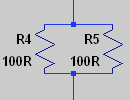
\includegraphics[width=.8\textwidth]{e04/Parallel.png}\footnotemark
    \end{center}
    \pause
    \column{.55\textwidth}
    \begin{block}{Berechnung}
      $$\frac{1}{R_{gesamt}} = \frac{1}{R_1} + \frac{1}{R_2} + \frac{1}{R_3} + ...$$
    \end{block}
  \end{columns}
  \footnotetext[1]{\tiny aus LTspice}
\end{frame}

\subsection{Ersatzwiderstand}
\begin{frame}
  \frametitle{Ersatzwiderstand}
  \begin{columns}
    \column{.47\textwidth}
    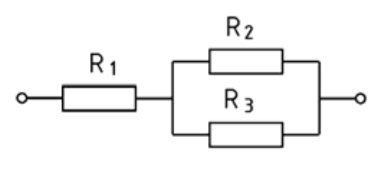
\includegraphics[width=1\textwidth]{e04/Ersatzwiderstand1.png}
    \column{.47\textwidth}
    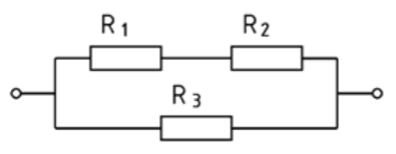
\includegraphics[width=1\textwidth]{e04/Ersatzwiderstand2.png}
  \end{columns}
  \begin{columns}
    \column{.47\textwidth}
    \pause
    \begin{exampleblock}{Berechnung}
      $R_1 + (R_2 \parallel R_3)$ \\[1.5em]
      $\Rightarrow R_1 + \cfrac{1}{\cfrac{1}{R_2} + \cfrac{1}{R_3}}$
    \end{exampleblock}
    \column{.47\textwidth}
    \pause
    \begin{exampleblock}{Berechnung}
      $(R_1 + R_2) \parallel R_3$\\[1.5em]
      $\Rightarrow \cfrac{1}{\cfrac{1}{R_1 + R_2} + \cfrac{1}{R_3}}$
    \end{exampleblock}
  \end{columns}
\end{frame}

\subsection{Spannungsteiler}
\begin{frame}
  \frametitle{Spannungsteiler}
  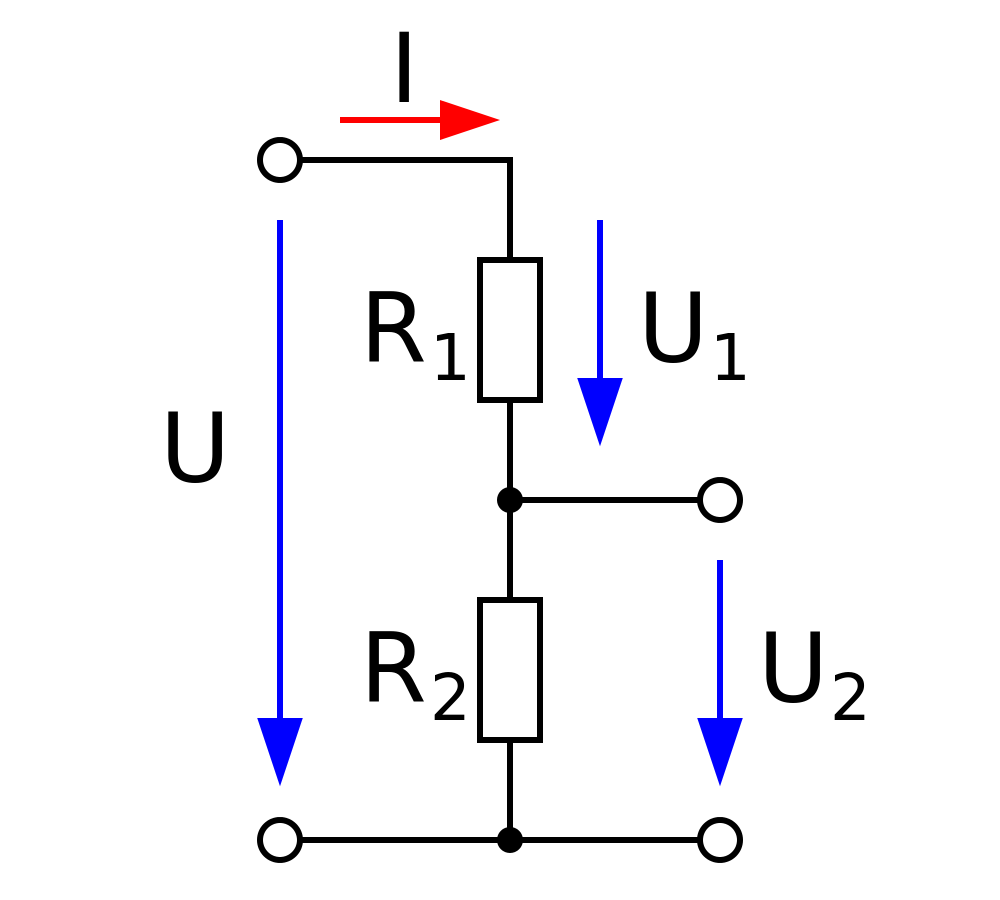
\includegraphics[scale=0.13]{a02/spannungsteiler-unbelastet.png}
  \hspace{2mm}
  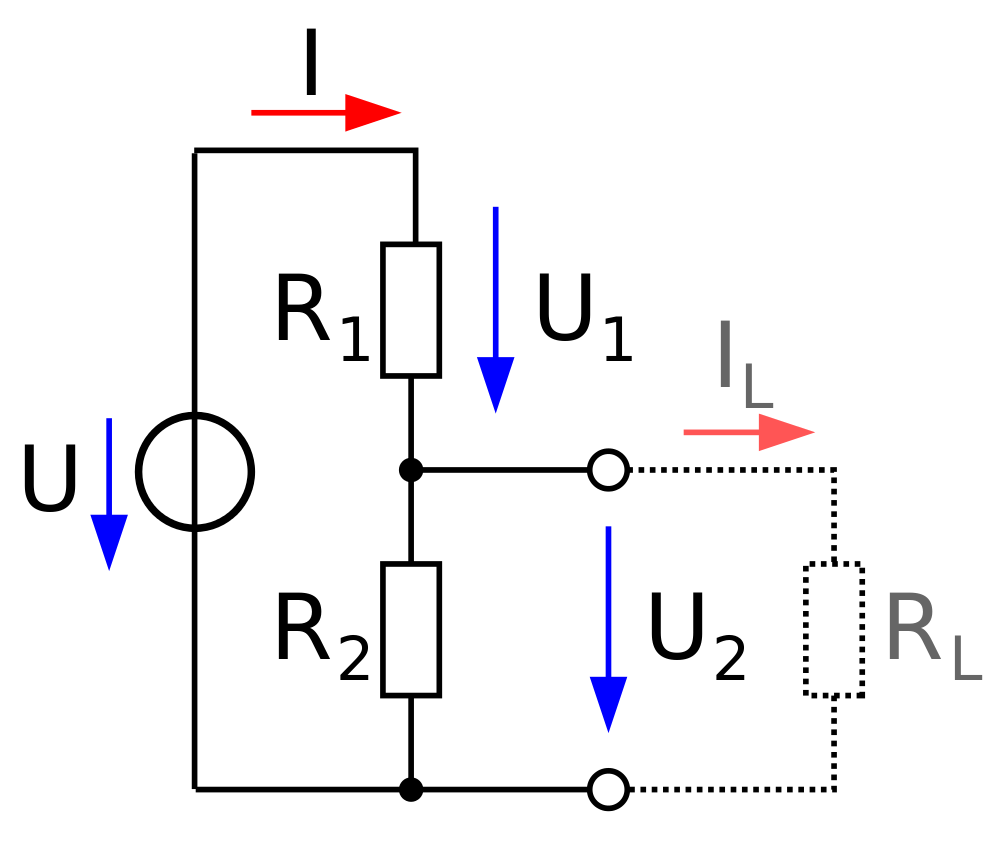
\includegraphics[scale=0.13]{a02/spannungsteiler-belastet.png}\\
  {\tiny Abb.9: Unbelasteter Spannungsteiler \cite{wp}}
  \hspace{10mm}
  {\tiny Abb.10: Belasteter Spannungsteiler \cite{wp}}
  \begin{itemize}
    \item $U_2$ ist beim belasteten Spannungsteiler kleiner als beim unbelasteten Spannungsteiler
  \end{itemize}
\end{frame}

\begin{frame}
  \frametitle{Rechnen beim Spannungsteiler}
  \textbf{beim unbelasteten Spannungsteiler:}
  \begin{itemize}
    \item $U_2$ ist die Spannung über $R_2$
  \end{itemize}
  \begin{block}{unbelasteter Spannungsteiler}
    \begin{center}
      $$\frac{U_2}{U} = \frac{R_2}{R_{gesamt}}$$
    \end{center}
  \end{block}

  \textbf{beim belasteten Spannungsteiler:}
  \begin{itemize}
    \item $U_2$ ist die Spannung über den beiden parallelen Widerstände $R_2$ und $R_L$
  \end{itemize}
  \begin{block}{belasteter Spannungsteiler}
    \begin{center}
      $$\frac{U_2}{U} = \frac{R_{2}||R_{L}}{R_{gesamt}}$$
    \end{center}
  \end{block}
\end{frame}

\section{Übung}

\begin{frame}
  \frametitle{Übungsaufgaben}

  Als Teil des Praxisskriptes im Anschluss.

\end{frame}

% \begin{frame}
%   \begin{tabular}{l||p{.8\textwidth}}\hline
%     \textbf{TB106} & \textbf{Was verstehen Sie unter Halbleitermaterialien?}\\ \hline\hline
%     A & Einige Stoffe (z.B. Silizium, Germanium) sind in reinem Zustand bei Zimmertemperatur gute Leiter. Durch geringfügige Zusätze von geeigneten anderen Stoffen nimmt jedoch ihre Leitfähigkeit ab. \\ \hline
%     B & Einige Stoffe wie z.B. Indium oder Magnesium sind in reinem Zustand bei Zimmertemperatur gute Isolatoren. Durch geringfügige Zusätze von Silizium, Germanium oder geeigneten anderen Stoffen werden sie jedoch zu Leitern. \\ \hline
%     C \only<2>\checkmark & Einige Stoffe (z.B. Silizium, Germanium) sind in reinem Zustand bei Zimmertemperatur gute Isolatoren. Durch geringfügige Zusätze von geeigneten anderen Stoffen oder bei hohen Temperaturen werden sie jedoch zu Leitern. \\ \hline
%     D & Einige Stoffe (z.B. Silizium, Germanium) sind in trockenem Zustand bei Zimmertemperatur gute Elektrolyten. Durch geringfügige Zusätze von Wismut oder Tellur kann man daraus entweder N-leitendes- oder P-leitendes Material für Anoden bzw. Katoden von Halbleiterbauelementen herstellen. \\ \hline
%   \end{tabular}
% \end{frame}
%
% \begin{frame}
%   \begin{tabular}{l||p{.8\textwidth}}\hline
%     \textbf{TB104} & \textbf{Der Temperaturkoeffizient für den Widerstand von metallischen Leitern ist \ldots}\\ \hline\hline
%     A & exponentiell \\ \hline
%     B & negativ \\ \hline
%     C & logarithmisch \\ \hline
%     D \only<2>\checkmark & positiv \\ \hline
%   \end{tabular}
% \end{frame}
%
%
% \begin{frame}
%   \begin{tabular}{l||p{.8\textwidth}}\hline
%     \textbf{TC109} & \textbf{Ein Widerstand hat eine Toleranz von 10 \%. Bei einem nominalen Widerstandswert von $5,6 k\Omega$ liegt der tatsächliche Wert zwischen}\\ \hline\hline
%     A \only<2>\checkmark & 5040 und 6160 $\Omega$ \\ \hline
%     B & 4760 und 6440 $\Omega$ \\ \hline
%     C & 4,7 und 6,8 $\Omega$ \\ \hline
%     D & 5,2 und 6,3 $\Omega$ \\ \hline
%   \end{tabular}
% \end{frame}
%
% \begin{frame}
%   \begin{tabular}{l||p{.8\textwidth}}\hline
% 		\textbf{TC112} & \textbf{Ein Lastwiderstand besteht aus zwölf parallel geschalteten 600-$\Omega$-Drahtwiderständen. Er eignet sich höchstens}\\ \hline\hline
% 		A & für Funkfrequenzen bis etwa 144 MHz.\\ \hline
% 		B & für UHF-Senderausgänge mit 50 $\Omega$.\\ \hline
% 		C \only<2>\checkmark & für Tonfrequenzen bis etwa 15 kHz.\\ \hline
% 		D & als Langdrahtersatz.\\ \hline
% 	\end{tabular}
% \end{frame}
%
% \begin{frame}
%   \begin{tabular}{l||p{.8\textwidth}}\hline
%     \textbf{TD302} & \textbf{Die Leerlaufspannung einer Gleichspannungsquelle beträgt 13,5 V. Wenn die Spannungsquelle einen Strom von 1 A abgibt, sinkt die Klemmenspannung auf 12,4 V. Wie groß ist der Innenwiderstand der Spannungsquelle?}\\ \hline\hline
%     A \only<2>\checkmark & $1,1 \Omega$\\ \hline
%     B & $1,2 \Omega$\\ \hline
%     C & $12,4 \Omega$\\ \hline
%     D & $13,5 \Omega$\\ \hline
%   \end{tabular}
%   \pause
%   \vspace{2em}
%   $$R = \frac{\Delta U}{\Delta I} = \frac{13,5V - 12,4V}{1A} = \frac{1,1V}{1A} = 1,1\Omega$$
% \end{frame}
%
% \begin{frame}
%   \begin{tabular}{l||p{.8\textwidth}}\hline
%     \textbf{TB102} & \textbf{Welchen Widerstand hat eine Kupferdrahtwicklung, wenn der verwendete Draht eine Länge von 1,8 m und einen Durchmesser von 0,2 mm hat?}\\ \hline\hline
%     A & $0,05 \Omega$\\ \hline
%     B \only<2>\checkmark &$1 \Omega$\\ \hline
%     C & $5,6 \Omega$\\ \hline
%     D & $56 \Omega$\\ \hline
%   \end{tabular}
%   \pause
%   \vspace{2em}
%   $$R = \frac{\rho \cdot \ell}{A_{Dr}}$$
%   \pause
%   $$A_{Dr} = \frac{d^2 \cdot \pi}{4} = \frac{0,2mm^2 \cdot \pi}{4} = 0,0314mm^2$$
%   \pause
%   $$\Rightarrow R = \frac{0,0178 \frac{\Omega \cdot mm^2}{m} \cdot 1,8m}{0,0314mm^2} = \frac{0,03204 \Omega}{0,0314} \approx 1\Omega$$
% \end{frame}
%
% \begin{frame}
%   \begin{tabular}{l||p{.8\textwidth}}\hline
%     \textbf{TB105} & \textbf{Welche Gruppe von Materialien enthält nur Nichtleiter?}\\ \hline\hline
%     A \only<2>\checkmark & Epoxyd, Polyethylen (PE), Polystyrol (PS)\\ \hline
%     B & Pertinax, Polyvinylchlorid (PVC), Graphit\\ \hline
%     C & Polyethylen (PE), Messing, Konstantan\\ \hline
%     D & Teflon, Pertinax, Bronze\\ \hline
%   \end{tabular}
% \end{frame}
%
% \begin{frame}
%   \begin{tabular}{l||p{.8\textwidth}}\hline
%     \textbf{TC103} & \textbf{Metalloxidwiderstände}\\ \hline\hline
%     A & haben geringe Toleranzen und Widerstandsänderungen und sind besonders als Präzisionswiderstände in der Messtechnik geeignet.\\ \hline
%     B & sind besonders als Hochlastwiderstände bei niedrigen Frequenzen geeignet.\\ \hline
%     C \only<2>\checkmark & sind induktionsarm und eignen sich besonders für den Einsatz bei sehr hohen Frequenzen.\\ \hline
%     D & haben einen extrem stark negativen Temperaturkoeffizienten und sind besonders als NTC-Widerstände (Heißleiter) geeignet.\\ \hline
%   \end{tabular}
% \end{frame}
%
% \begin{frame}
%   \begin{tabular}{l||p{.8\textwidth}}\hline
%     \textbf{TD301} & \textbf{Welche Eigenschaften sollten Strom- und Spannungsquellen aufweisen?}\\ \hline\hline
%     A & Strom- und Spannungsquellen sollten einen möglichst niedrigen Innenwiderstand haben.\\ \hline
%     B & Strom- und Spannungsquellen sollten einen möglichst hohen Innenwiderstand haben.\\ \hline
%     C & Spannungsquellen sollten einen möglichst hohen Innenwiderstand und Stromquellen einen möglichst niedrigen Innenwiderstand haben.\\ \hline
%     D \only<2>\checkmark & Spannungsquellen sollten einen möglichst niedrigen Innenwiderstand und Stromquellen einen möglichst hohen Innenwiderstand haben.\\ \hline
%   \end{tabular}
% \end{frame}
%
% \begin{frame}
%   \begin{tabular}{l||p{.8\textwidth}}\hline
%     \textbf{TB914} & \textbf{Welche Belastbarkeit muss ein 100-Ohm-Widerstand, an dem 10 Volt anliegen, mindestens haben?}\\ \hline\hline
%     A & 100 mW\\ \hline
%     B & 0,125 W\\ \hline
%     C \only<2>\checkmark & 1 W\\ \hline
%     D & 10 W \\ \hline
%   \end{tabular}
%   \pause
%   \vspace{2em}
%   $$P = \frac{U^2}{R} = \frac{10V^2}{100\Omega} = 1W$$
% \end{frame}
%
% \begin{frame}
%   \begin{tabular}{l||p{.8\textwidth}}\hline
%     \textbf{TB923} & \textbf{In welcher Antwort sind alle dargestellten Zusammenhänge zwischen Strom, Spannung, Widerstand und Leistung richtig?}\\ \hline\hline
%     A & $$I = \sqrt{P \cdot R} \:,\: U = \sqrt{\frac{P}{R}}$$\\ \hline
%     B & $$I = \sqrt{\frac{R}{P}} \:,\: U = \sqrt{P \cdot R}$$\\ \hline
%     C \only<2>\checkmark & $$I = \sqrt{\frac{P}{R}} \:,\: U = \sqrt{P \cdot R}$$\\ \hline
%     D & $$I = \frac{\sqrt{P}}{P} \:,\: U = \sqrt{P} \cdot R$$\\ \hline
%   \end{tabular}
% \end{frame}
%
% \begin{frame}
%   \begin{exampleblock}{Weitere Übungen}
%     TD107--TD108, TD111--TD115, TD121--TD124, TJ708
%   \end{exampleblock}
% \end{frame}

\section{Referenzen}
\begin{small}
  \begin{thebibliography}{}
      \setbeamertemplate{bibliography item}[online]
    \bibitem{a02}  Moltrecht A 02: \\
      \url{http://www.darc.de/referate/ajw/ausbildung/darc-online-lehrgang/technik-klasse-a/technik-a02/}

    \bibitem{wp}    Wikipedia DE: \\
      \url{http://de.wikipedia.org/wiki/Spannungsteiler}\\
      \url{http://de.wikipedia.org/wiki/Datei:Einfacher-unbelasteter-Spannungsteiler.svg}\\
      \url{http://de.wikipedia.org/wiki/Datei:Einfacher-Spannungsteiler.svg}\\
      \url{http://de.wikipedia.org/wiki/Ohmsches_Gesetz}\\
      \url{http://de.wikipedia.org/wiki/Elektrische_Leistung}\\
      \url{http://de.wikipedia.org/wiki/lektrische_Energie#Elektrische_Energie_in_einem_elektrischen_Feld}\\

    \bibitem{wmde}	Wikimedia DE:\\
      \url{http://commons.wikimedia.org/wiki/File:Ohmsches_Gesetz.svg?uselang=de}\\
    \bibitem{wmen}	Wikimedia EN:\\
      \url{http://commons.wikimedia.org/wiki/File:Ohm\%27s_law_triangle.PNG}
  \end{thebibliography}
\end{small}

% Hier könnte noch eine Kontaktfolie stehen

\end{document}

